% Native editable composition from verified, unchanged IDE images.
\par
\begin{figure}[htbp]
\centering
\sbox0{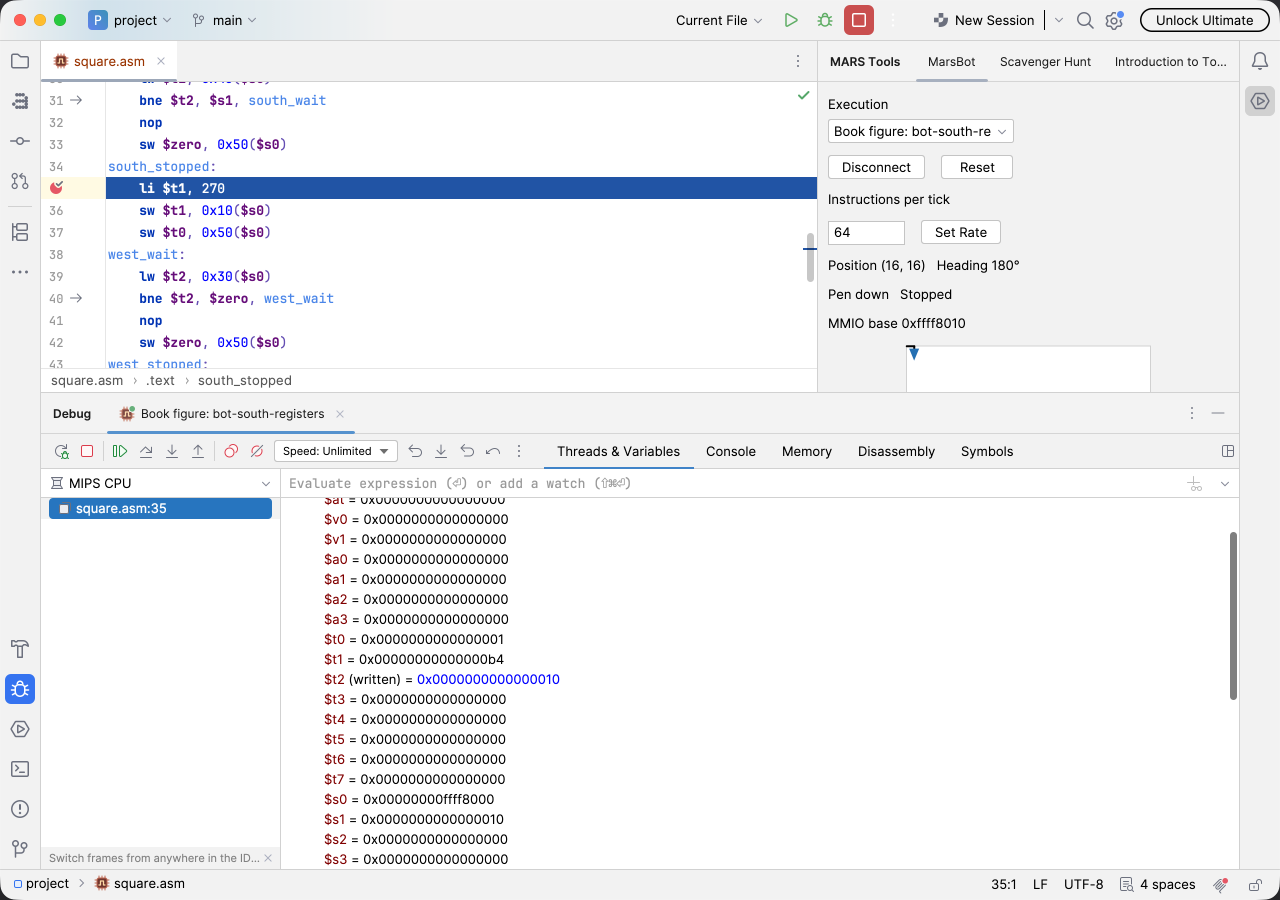
\includegraphics[artifact]{book/captures/006-marsbot-square/f02-south/registers.png}}
\sbox2{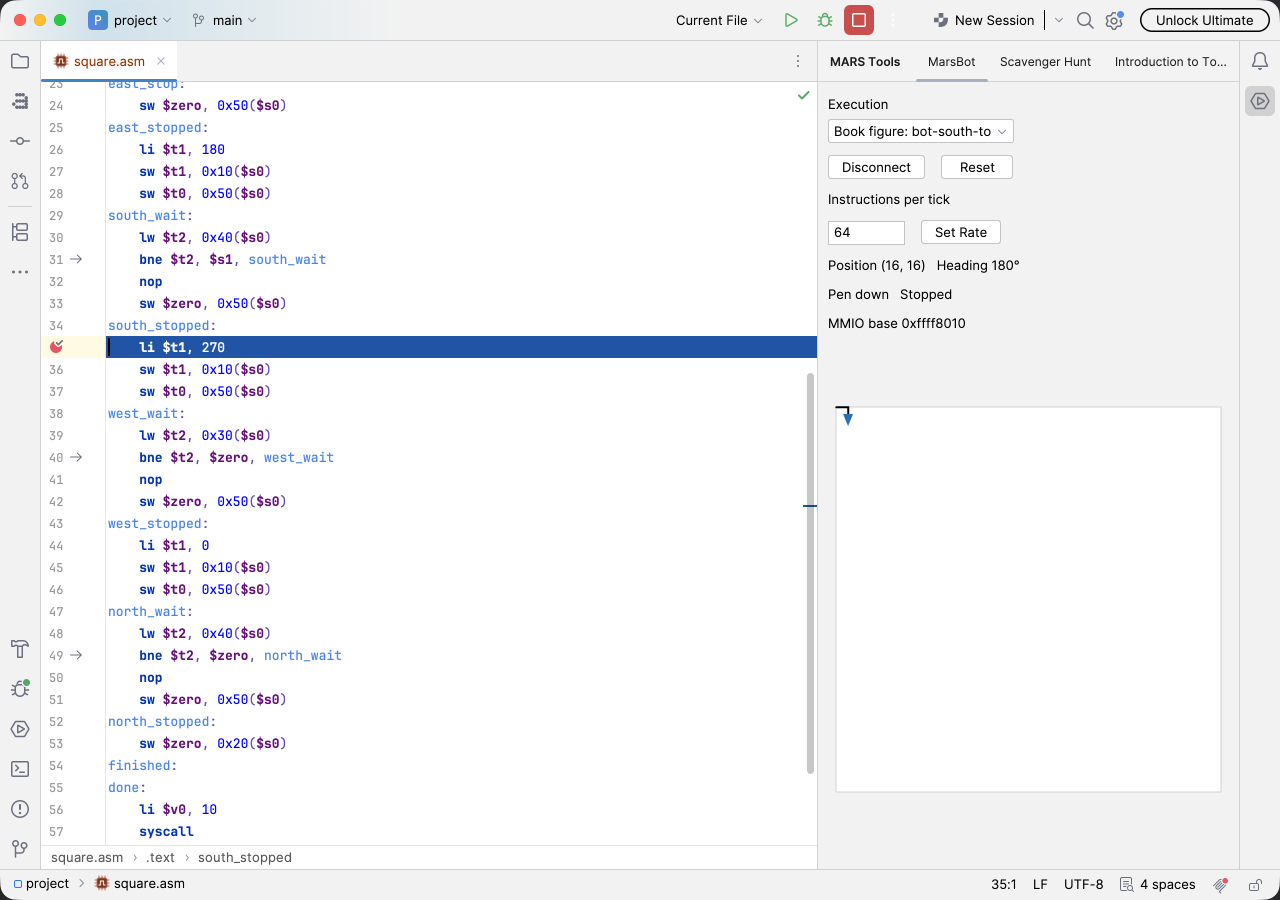
\includegraphics[artifact]{book/captures/006-marsbot-square/f02-south/tool.png}}
\edef\MARSsouthsourceLeft{\the\dimexpr0.036718750\wd0\relax}
\edef\MARSsouthsourceBottom{\the\dimexpr0.774444444\ht0\relax}
\edef\MARSsouthsourceRight{\the\dimexpr0.611718750\wd0\relax}
\edef\MARSsouthsourceTop{\the\dimexpr0.147777778\ht0\relax}
\edef\MARSsouthstatusLeft{\the\dimexpr0.641406250\wd2\relax}
\edef\MARSsouthstatusBottom{\the\dimexpr0.658888889\ht2\relax}
\edef\MARSsouthstatusRight{\the\dimexpr0.186718750\wd2\relax}
\edef\MARSsouthstatusTop{\the\dimexpr0.215555556\ht2\relax}
\edef\MARSsouthregistersLeft{\the\dimexpr0.246093750\wd0\relax}
\edef\MARSsouthregistersBottom{\the\dimexpr0.075555556\ht0\relax}
\edef\MARSsouthregistersRight{\the\dimexpr0.556250000\wd0\relax}
\edef\MARSsouthregistersTop{\the\dimexpr0.740000000\ht0\relax}
\edef\MARSsouthtrailLeft{\the\dimexpr0.646875000\wd2\relax}
\edef\MARSsouthtrailBottom{\the\dimexpr0.522222222\ht2\relax}
\edef\MARSsouthtrailRight{\the\dimexpr0.328906250\wd2\relax}
\edef\MARSsouthtrailTop{\the\dimexpr0.441111111\ht2\relax}
\begin{tikzpicture}[alt={Four annotated details at south stopped. The next instruction loads 270 into t1. The native tool reports position sixteen sixteen, heading 180 degrees, pen down and stopped, at sixty-four instructions per tick. Register t2 and target s1 both equal sixteen. An enlarged original board crop shows the rightward then downward pen trail and a downward-pointing marker.}]
\node[anchor=north west,inner sep=0,font=\small\bfseries] (source-title) at (6mm,0) {Prepare the west heading after stopping};
\node[anchor=north west,inner sep=0] (source) at ([yshift=-1mm]source-title.south west) {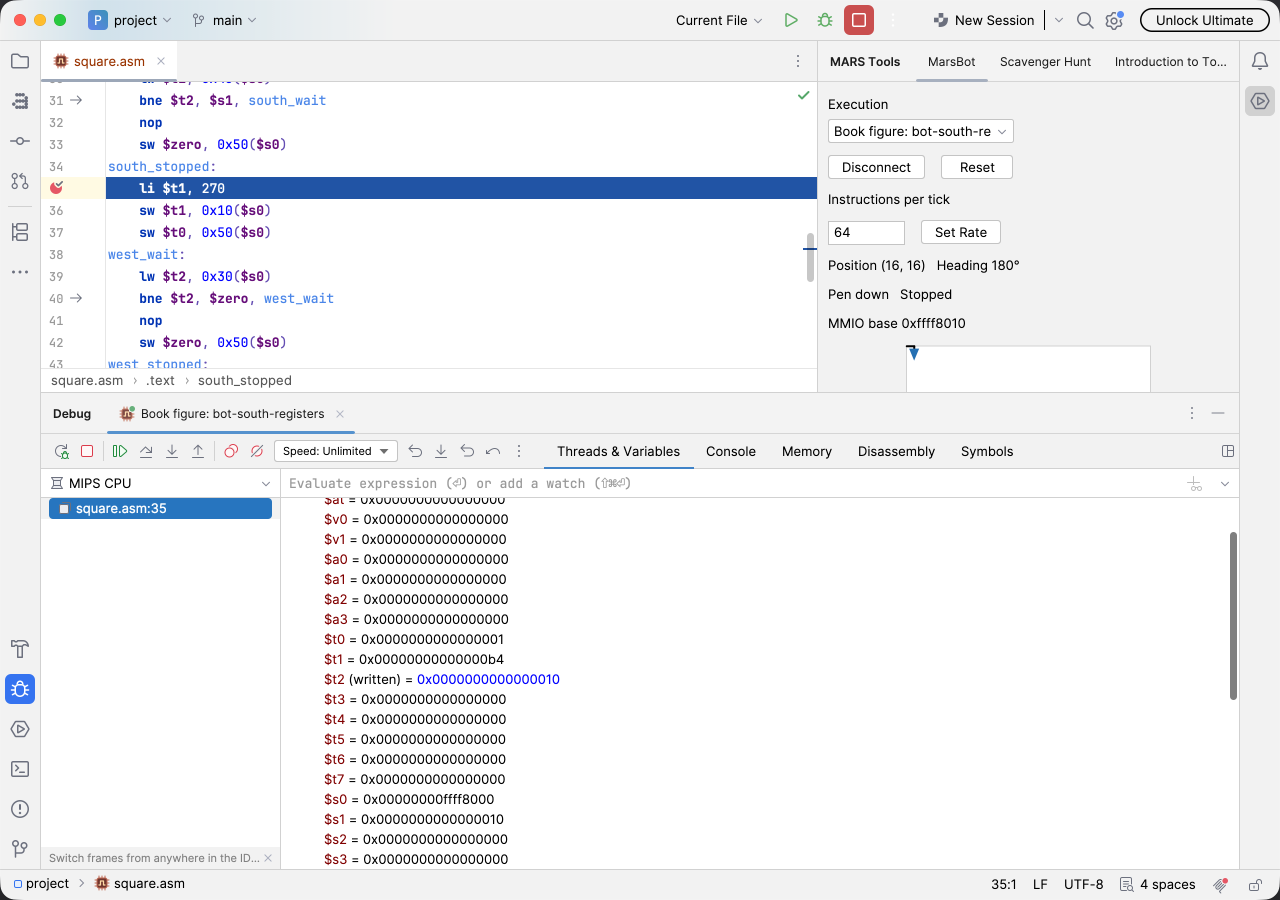
\includegraphics[width=0.7\linewidth,artifact,trim={\MARSsouthsourceLeft{} \MARSsouthsourceBottom{} \MARSsouthsourceRight{} \MARSsouthsourceTop{}},clip]{book/captures/006-marsbot-square/f02-south/registers.png}};
\begin{scope}[shift={(source.south west)},x={($(source.south east)-(source.south west)$)},y={($(source.north west)-(source.south west)$)}]
\draw[black,line width=0.7pt] (0.135555556,0.057142857) rectangle (0.395555556,0.371428571);
\node[draw=black,fill=white,circle,inner sep=1.5pt,font=\footnotesize] at ($(0.135555556,0.371428571)+(-3mm,0)$) {1};
\end{scope}
\node[anchor=north west,inner sep=0,font=\small\bfseries] (status-title) at ([yshift=-2mm]source.south west) {The south leg increased the y coordinate};
\node[anchor=north west,inner sep=0] (status) at ([yshift=-1mm]status-title.south west) {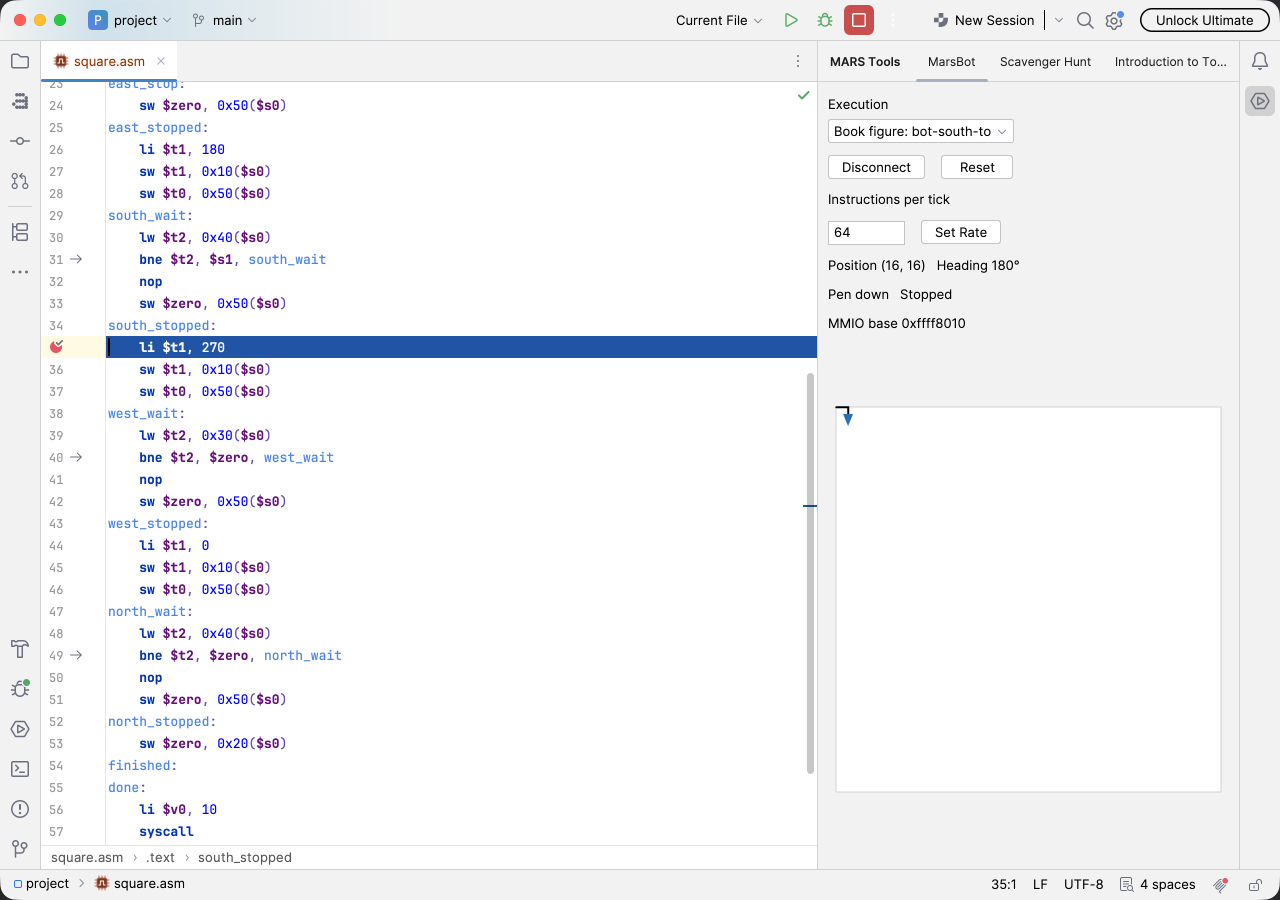
\includegraphics[width=0.4\linewidth,artifact,trim={\MARSsouthstatusLeft{} \MARSsouthstatusBottom{} \MARSsouthstatusRight{} \MARSsouthstatusTop{}},clip]{book/captures/006-marsbot-square/f02-south/tool.png}};
\begin{scope}[shift={(status.south west)},x={($(status.south east)-(status.south west)$)},y={($(status.north west)-(status.south west)$)}]
\draw[black,line width=0.7pt] (0.018181818,0.035398230) rectangle (0.904545455,0.787610619);
\node[draw=black,fill=white,circle,inner sep=1.5pt,font=\footnotesize] at ($(0.019704433,0.787610619)+(-3mm,0)$) {2};
\end{scope}
\node[anchor=north west,inner sep=0,font=\small\bfseries] (trail-title) at ([xshift=0.48\linewidth]status-title.north west) {Enlarged board detail};
\node[anchor=north west,inner sep=0] (trail) at ([yshift=-1mm]trail-title.south west) {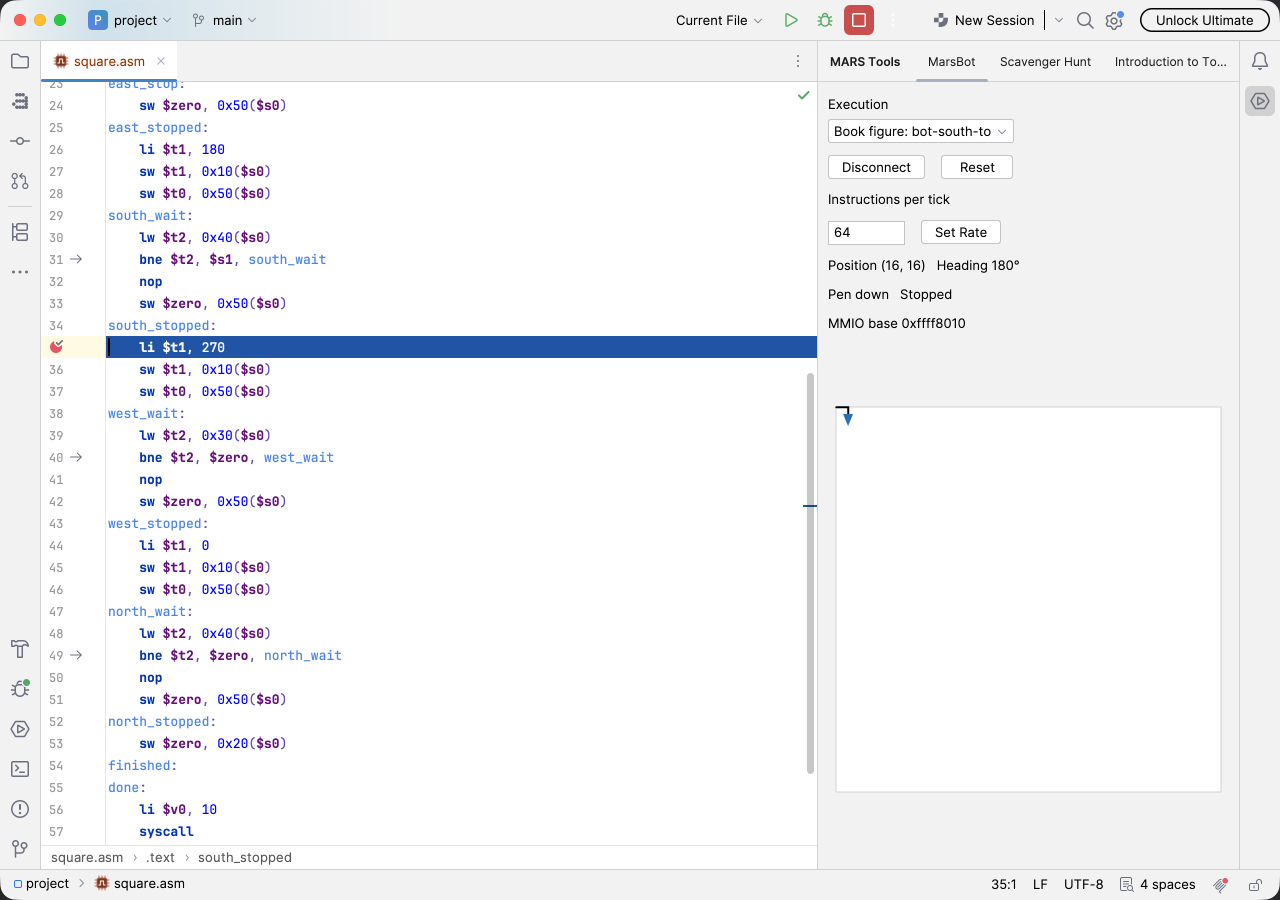
\includegraphics[width=0.16\linewidth,artifact,trim={\MARSsouthtrailLeft{} \MARSsouthtrailBottom{} \MARSsouthtrailRight{} \MARSsouthtrailTop{}},clip]{book/captures/006-marsbot-square/f02-south/tool.png}};
\begin{scope}[shift={(trail.south west)},x={($(trail.south east)-(trail.south west)$)},y={($(trail.north west)-(trail.south west)$)}]
\draw[black,line width=0.7pt] (0.000000000,0.000000000) rectangle (1.000000000,1.000000000);
\node[draw=black,fill=white,circle,inner sep=1.5pt,font=\footnotesize] at ($(0.000000000,1.000000000)+(-3mm,0)$) {3};
\end{scope}
\node[anchor=north west,inner sep=0,font=\small\bfseries] (registers-title) at ([yshift=-2mm]status.south west) {This equality used y feedback};
\node[anchor=north west,inner sep=0] (registers) at ([yshift=-1mm]registers-title.south west) {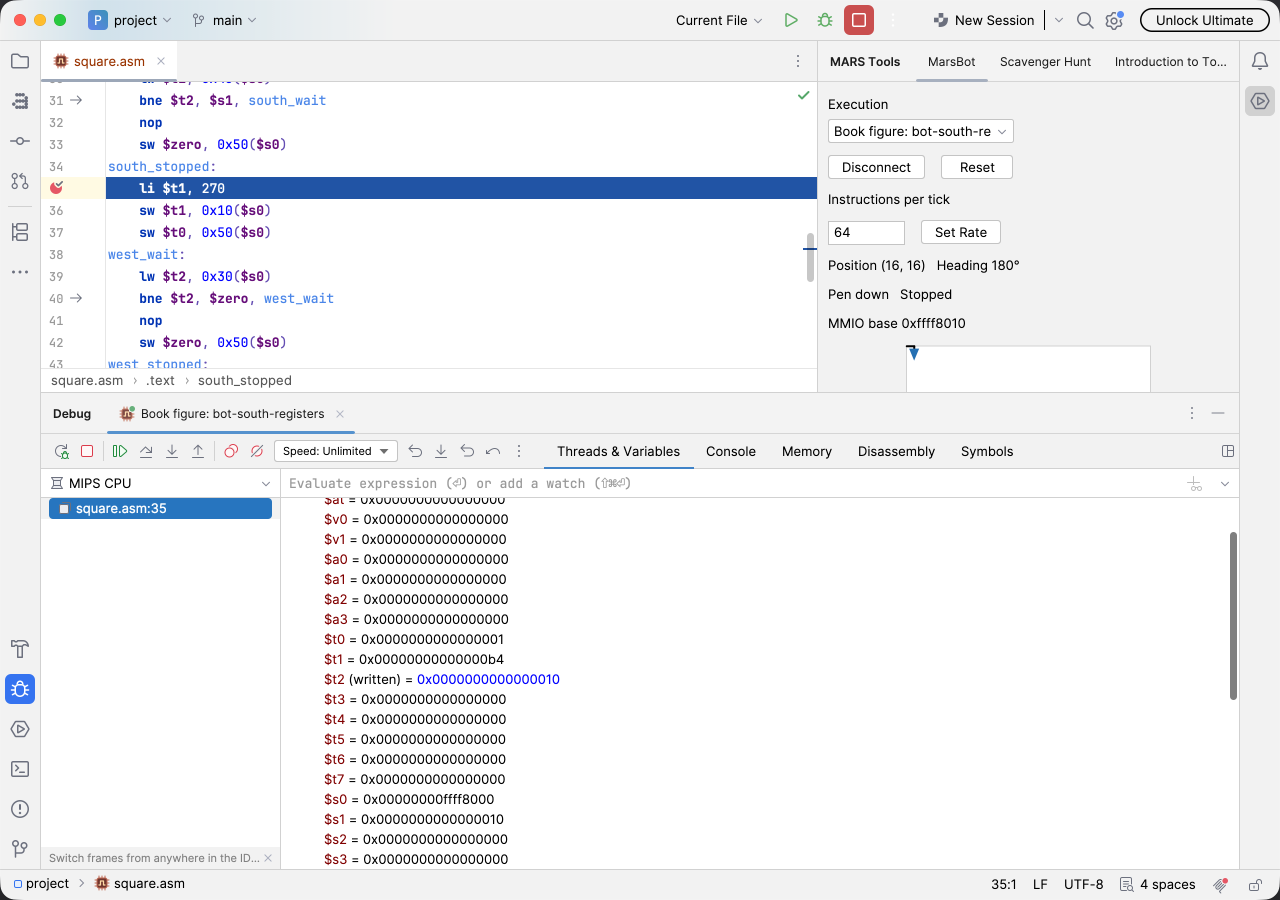
\includegraphics[width=0.36\linewidth,artifact,trim={\MARSsouthregistersLeft{} \MARSsouthregistersBottom{} \MARSsouthregistersRight{} \MARSsouthregistersTop{}},clip]{book/captures/006-marsbot-square/f02-south/registers.png}};
\begin{scope}[shift={(registers.south west)},x={($(registers.south east)-(registers.south west)$)},y={($(registers.north west)-(registers.south west)$)}]
\draw[black,line width=0.7pt] (0.023715415,0.018072289) rectangle (0.976284585,0.981927711);
\node[draw=black,fill=white,circle,inner sep=1.5pt,font=\footnotesize] at ($(0.023715415,0.981927711)+(-3mm,0)$) {4};
\end{scope}
\end{tikzpicture}
\par\smallskip
\begin{minipage}{\linewidth}
\small
\begin{enumerate}
\item The next \texttt{li \$t1, 270} prepares the west leg. The preceding movement-port store is complete, so the device is already stopped. A constant in a CPU register becomes a device command only when the following port store executes.
\item Position is $(16,16)$ and heading is $180^\circ$. The pen is still down. Positive $y$ points down on this board, so the second leg moved toward the lower-right corner while keeping $x=16$. The clock setting remains 64 instructions per tick.
\item The enlarged original crop shows $(0,0)\rightarrow(16,0)\rightarrow(16,16)$. The arrow now points down at the second endpoint. The first corner remains in the pen history; it is not redrawn by the chapter annotation. The coordinate sequence supplies the same information without relying on color.
\item \texttt{\$t2}=\texttt{\$s1}=16 here compares the loaded \emph{y} coordinate with the same side-length target. The south loop reads offset \texttt{0x40}; the east loop read offset \texttt{0x30}. Changing only the heading would leave the wrong feedback test in place.
\end{enumerate}
\end{minipage}
\caption{The second side is stopped at the lower-right corner. The heading and the coordinate being polled changed between the two legs.}
\label{capture:006-marsbot-square-f02-south}
\end{figure}
\par
